\documentclass{article}
\usepackage{graphicx} % Required for inserting images
\usepackage{amsmath,amssymb,amsfonts,textcomp}
\usepackage{float,flafter}
\usepackage{hyperref}
\usepackage{inputenc}
\usepackage{xcolor}
\usepackage{listings} % Corrected from listing to listings
\usepackage{adjustbox}
\usepackage{pifont} % For checkmarks in the document
\usepackage{tikz} % For decorative elements
\usepackage{geometry}
\usepackage{fancyhdr} % For header and footer customization
\usepackage[authoryear]{natbib} % For textcite - Important: Keep this for textcite to work

\lstdefinestyle{verilog-style}{
  language=Verilog,
  basicstyle=\ttfamily\small,
  keywordstyle=\color{blue},
  commentstyle=\color{green!50!black},
  stringstyle=\color{red},
  numbers=left,
  numberstyle=\tiny\color{gray},
  numbersep=5pt,
  breaklines=true,
  showstringspaces=false,
  frame=single,
  tabsize=2
}
\lstset{
  literate={~}{{\textasciitilde}}1
}
\numberwithin{figure}{section}
\numberwithin{table}{section}
% Page geometry
\geometry{a4paper,top=2cm,bottom=2cm,left=3cm,right=3cm,marginparwidth=1.75cm}
% Hyperref setup
\hypersetup{
    colorlinks=true,
    linkcolor=blue,
    filecolor=magenta,
    urlcolor=cyan,
}
% Define colors
\definecolor{titlecolor}{RGB}{25,55,100}
\definecolor{accentcolor}{RGB}{70,130,180}
\title{IPA Course Project}
\author{Hrishikesh Milind Gawas, Vignesh Vembar, Krish Pandya}
\date{\today}
% Custom header and footer
\pagestyle{fancy}
\fancyhf{}
\fancyhead[L]{IPA Course Project}
\fancyhead[R]{64-bit RISC V Processor}
\fancyfoot[C]{\thepage}
\renewcommand{\headrulewidth}{0.4pt}
\renewcommand{\footrulewidth}{0.4pt}
\begin{document}


\begin{titlepage}
    \begin{tikzpicture}[remember picture, overlay]
        % Background - modern light gray
        \fill[color=gray!5] (current page.north west) rectangle (current page.south east);
        
        % Top and bottom bars - sleek blue gradient
        \shade[left color=cyan!30, right color=blue!60] (current page.north west) rectangle ([yshift=-0.4cm]current page.north east);
        \shade[left color=blue!60, right color=cyan!30] (current page.south west) rectangle ([yshift=0.4cm]current page.south east);
    \end{tikzpicture}
    
    \centering
    \vspace*{1cm}
    \rule{\linewidth}{0.6mm}
    \vspace{0.1cm}
    {\Huge\bfseries\textcolor{blue!70}{Course Project Report}\par}
    \vspace{0.5cm}
    \rule{\linewidth}{0.6mm}
    
    \vspace{1.5cm}
    {\Large\bfseries \textit{Introduction to Processor Architecture}\par}
    
    \vspace{1.8cm}
    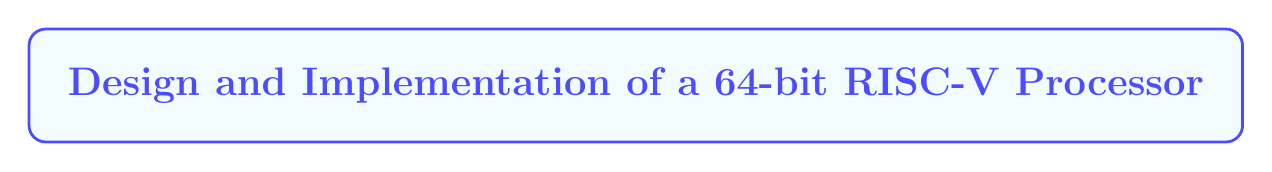
\begin{tikzpicture}
        \node[draw=blue!70, rounded corners=6pt, line width=1pt, inner sep=14pt, fill=cyan!5]
            {\Large\bfseries\textcolor{blue!70}{Design and Implementation of a 64-bit RISC-V Processor}};
    \end{tikzpicture}
    
    \vspace{2.0cm}
    {\large\textbf{Abstract:}\par}
    \vspace{0.5cm}
    \noindent This report describes the design and implementation of a 64-bit RISC-V processor with pipeline and hazard detection. The processor is implemented in Verilog and can execute a subset of the RISC-V instruction set. The processor is pipelined to improve performance, and it includes hazard detection logic to prevent data hazards and control hazards. The processor is also equipped with a branch predictor to reduce the performance impact of control hazards.
    
    \vspace{2cm}
    {\large\textbf{Submitted by:}\par}
    
    \vspace{0.8cm}
    \fbox{\begin{minipage}{0.9\linewidth}
        \centering
        \begin{tabular}{c c c}
            \large Hrishikesh Milind Gawas & \large Vignesh Vembar & \large Krish Pandya \\
            \textcolor{gray!99}{2024122006} & \textcolor{gray!99}{2023102019} & \textcolor{gray!99}{2023102026}
        \end{tabular}
    \end{minipage}}
    
    \vfill
    {\Large\bfseries Academic Year: 2024 - 2025\par}
    \vspace{1.2cm}
\end{titlepage}




\newpage
\tableofcontents
\thispagestyle{fancy}
\newpage
\setcounter{section}{0}
\section{Sequential CPU Design}
\subsection{Overview}
The \texttt{cpu\_sequential} module is the final wrapper module which features a \textbf{basic 64-bit RISC-V processor} designed to execute instructions sequentially. It includes key components such as the \textbf{program counter (PC), instruction memory, control unit, register file, ALU, and data memory}, which work together to execute instructions in a step-by-step manner.
\subsection{Working of the CPU}
The CPU follows the standard \textbf{instruction execution cycle}, which consists of the following stages:
\begin{itemize}
    \item Instruction Fetch
    \item Instruction Decode
    \item Execute
    \item Memory Access
    \item Write-back
\end{itemize}
\subsubsection*{1. Instruction Fetch}
\begin{itemize}
    \item Features a 64-bit program counter which holds the address of the current instruction. This updates at every positive clock edge to point to the next instruction or branch target.
    \item Features separate memory for instruction and data storage. This prevents data hazards, discussed in later sections.
    \item Fetches the instruction from the \textbf{instruction memory} using the \texttt{pc\_current} value.
\end{itemize}
\subsubsection*{2. Instruction Decode}
\begin{itemize}
    \item Features \textbf{control unit} which decodes the instruction and generates control signals. These determine the type of operation such as memory operations, arithmetic operations, and branch execution.
    \item Features a \textbf{register bank} which provides data stores on two source registers (\texttt{rs1} and \texttt{rs2}). This unit also writes the computed result to the destination register (\texttt{rd}).
\end{itemize}
\begin{figure}[H]
    \centering
    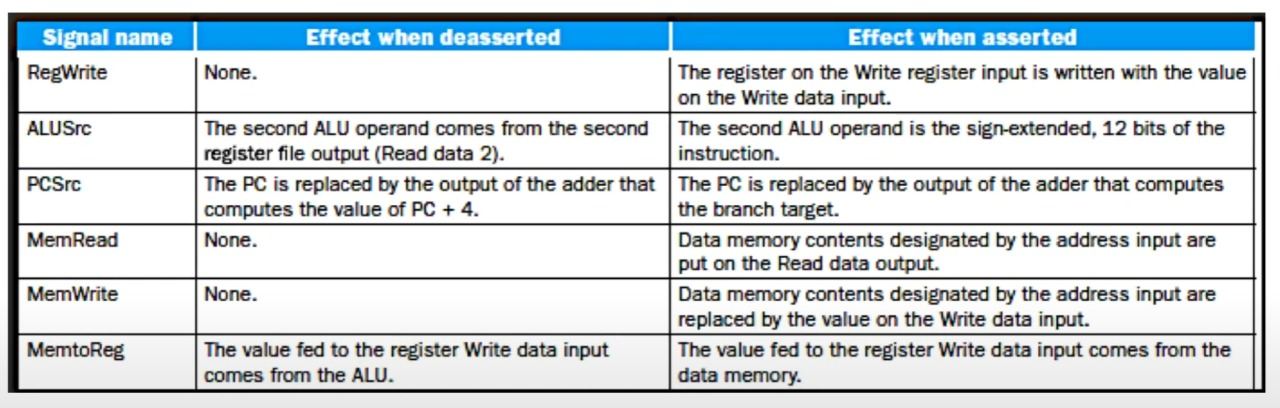
\includegraphics[width=1.0\linewidth]{Control_Signals.jpg}
    \caption{Control Signals}
    \label{fig:control-signals}
\end{figure}
\subsubsection*{3. Execute}
\begin{itemize}
    \item Features ALU (Arithmetic Logic Unit) which performs arithmetic and logical operations. It takes two inputs \texttt{reg\_read\_data1} (First operand) and \texttt{alu\_operand2} (Second operand - register or immediate value) and produces \texttt{alu\_result} and the \texttt{zero} flag (useful for branch instruction \textit{beq}).
    \item This processor supports a subset of RISC-V instructions:
        \begin{itemize}
            \item R-type: add, sub, or, and
            \item I-type: addi, ld (load doubleword)
            \item S-type: sd (store doubleword)
            \item SB-type: beq (branch if equal)
            \item Special: nop (no operation)
        \end{itemize}
    \item If a branch instruction is executed, the \texttt{zero} flag determines whether to take the branch. The new PC address is calculated and provided to the multiplexer before \texttt{pc\_next}. If no branch is taken, the PC increments sequentially (PC+4).
\end{itemize}
\subsubsection*{4. Memory Access}
\begin{itemize}
    \item Load instructions (\texttt{ld}) fetch data from \textbf{data memory} and Store instructions (\texttt{sd}) write data to memory.
\end{itemize}
\subsubsection*{5. Write-back}
\begin{itemize}
    \item The final result is written back to the register file. The value comes from either memory or the ALU result which is set using the \texttt{mem\_to\_reg} control signal.
\end{itemize}
\begin{figure}[H]
    \centering
    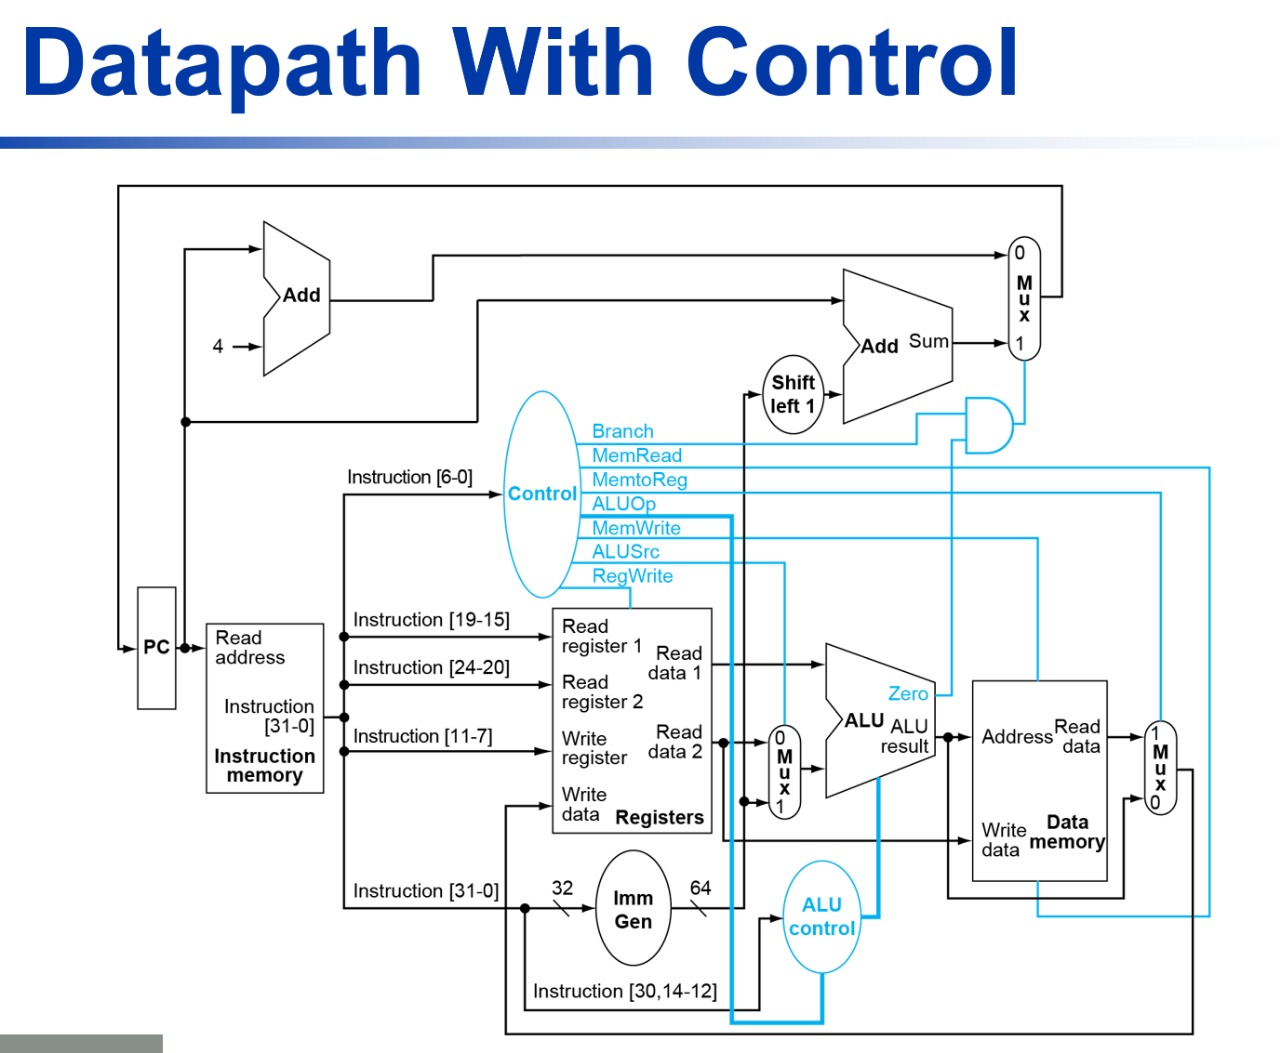
\includegraphics[width=1\linewidth]{Sequential_datapath_control.jpg}
    \caption{Sequential Datapath and Control Logic}
    \label{fig:sequential-datapath}
\end{figure}
\subsection{Assembler}
\subsubsection{Introduction}
An \textbf{assembler} is a program that translates assembly language instructions into machine code (binary format). The assembler processes RISC-V assembly instructions and generates corresponding binary instructions to be loaded into the instruction memory of the CPU.
\subsubsection{Assembler Overview}
The assembler operates in two passes:
\begin{enumerate}
\item \textbf{First Pass: Label Collection}
\begin{itemize}
\item Reads the assembly file and scans for labels (used in branching instructions).
\item Assigns memory addresses to labels so they can be referenced later.
\end{itemize}
\item \textbf{Second Pass: Instruction Translation}
\begin{itemize}
\item Converts each assembly instruction into its binary format based on the RISC-V instruction set.
\item Uses predefined opcode, function codes (\texttt{funct3}, \texttt{funct7}), and register encoding.
\item Replaces label references with corresponding memory addresses.
\end{itemize}
\end{enumerate}
The output of this assembler is a list of \textbf{binary instructions} formatted in Verilog format, which is then inserted into the testbench.
\subsubsection{Testbench Generation}
The assembler generates a \textbf{testbench} in Verilog to verify the correctness of the \texttt{cpu\_sequential} module. The testbench:
\begin{itemize}
\item Initializes a clock signal (\texttt{clk}) with a 10ns period.
\item Generates a \textbf{reset} signal at the beginning to initialize the CPU.
\item Loads the generated machine instructions into the \textbf{instruction memory} (\texttt{imem}).
\item Simulates execution by stepping through the instruction cycle. The simulation runs until the CPU encounters an all zero bit \textbf{NOP (halt)} instruction.
\item Monitors CPU behavior, registers, and memory operations at every cycle which can be viewed on terminal as shown below.
\begin{figure}[H]
    \centering
    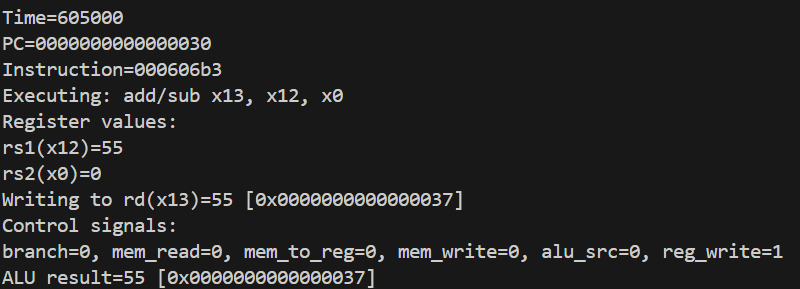
\includegraphics[width=1\linewidth]{test_bench_monitor.png}
    \caption{Cycle wise monitoring}
    \label{fig:test-bench}
\end{figure}
\item After execution, the testbench prints the final values of \textbf{registers} and \textbf{memory}. It also writes memory contents to a file (\texttt{data\_memory.hex}).
\item This measures the \textbf{execution time} of the program in cycles.
\end{itemize}
Finally, a bash script is written which integrates all files such as assembler, testbench generated and all the modules to simulate the results in one go!
\subsection{Simulation}
\subsubsection*{Case I}
Initially, a basic assembly sketch is implemented to test whether all functions work properly.
\begin{figure}[H]
    \centering
    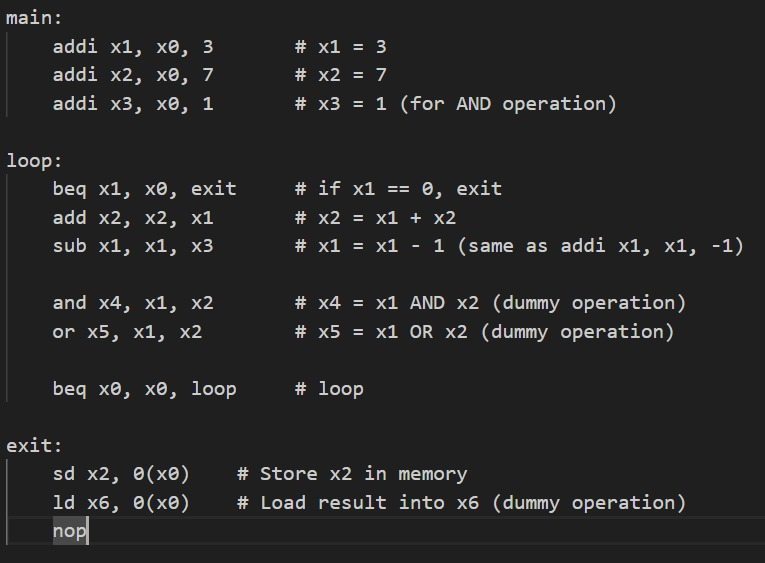
\includegraphics[width=1\linewidth]{basic_test_sequential.jpg}
    \caption{Basic Assembly}
    \label{fig:basic-test}
\end{figure}
\begin{figure}[H]
    \centering
    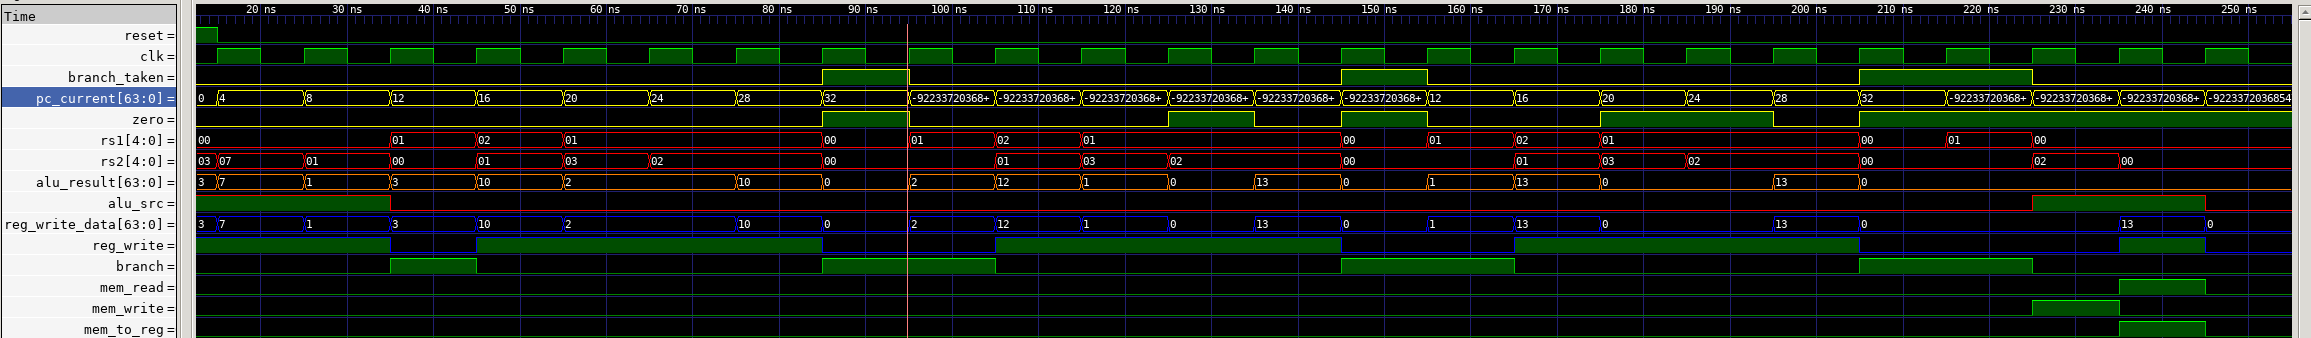
\includegraphics[width=1\linewidth]{Basic_sequential_test_gtkwave.png}
    \caption{GTKWave Output}
    \label{fig:gtkwave-output}
\end{figure}
\subsubsection*{Case II}
Some lengthy test cases were run to check edge cases.
\begin{figure}[H]
    \centering
    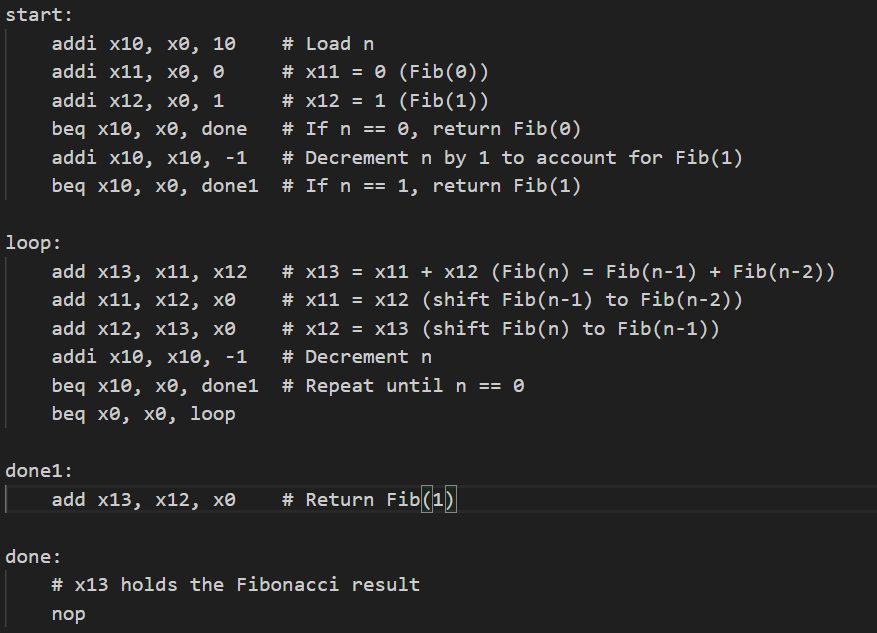
\includegraphics[width=1\linewidth]{Sequential_fibonacci.png}
    \caption{$n^{th}$ Fibonacci number}
    \label{fig:fibonacci}
\end{figure}
\begin{figure}[H]
    \centering
    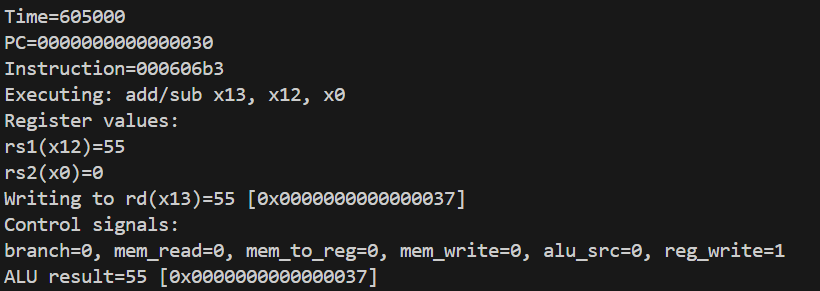
\includegraphics[width=1\linewidth]{Fibonacci_final_instruction.png}
    \caption{Final Instruction Output}
    \label{fig:fibonacci-output}
\end{figure}
\begin{figure}[H]
    \centering
    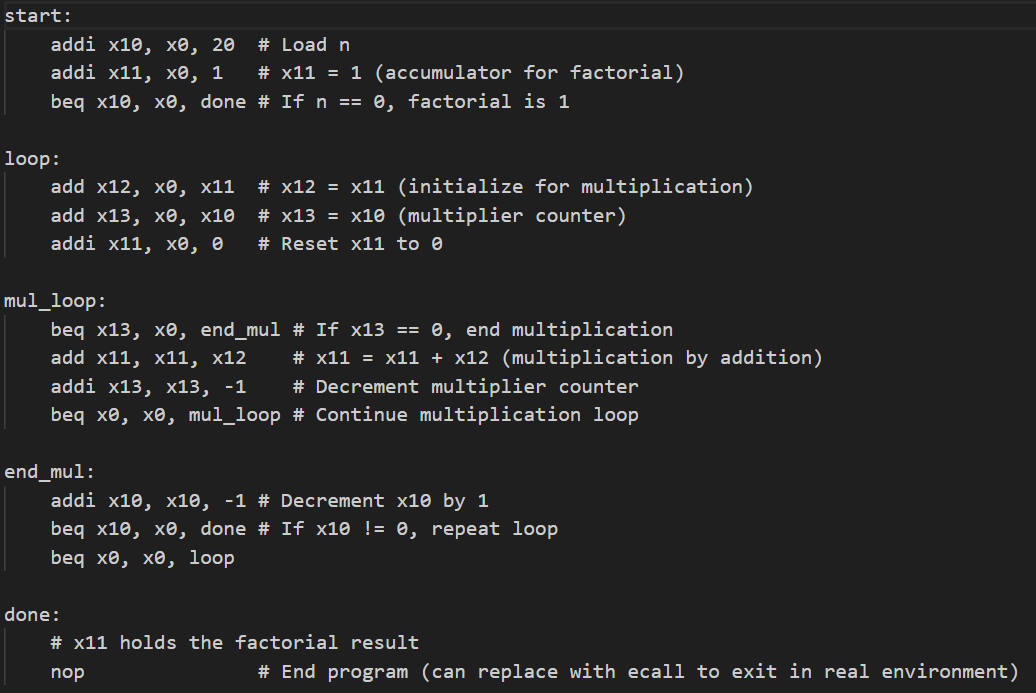
\includegraphics[width=1\linewidth]{sequential_factorial.png}
    \caption{$n^{th}$ Factorial}
    \label{fig:factorial}
\end{figure}
\begin{figure}[H]
    \centering
    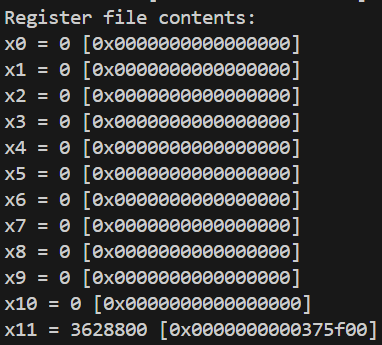
\includegraphics[width=0.6\linewidth]{seq_fac_out.png}
    \caption{Final Register Content (x11)}
    \label{fig:factorial-output}
\end{figure}
\subsection{Visualisation}
To enhance understanding of the CPU's operation, we developed a visualization tool that renders the processor's architectural components and data flow in real time. This interactive interface depicts the key components of the CPU including the register file, ALU, memory units, and control paths, allowing observation of instruction execution at each stage. Our visualization approach provides intuitive insights into the processor's behavior by highlighting active data paths and changing register values during program execution, making it especially valuable for debugging and educational purposes.

\begin{figure}[H]
    \centering
    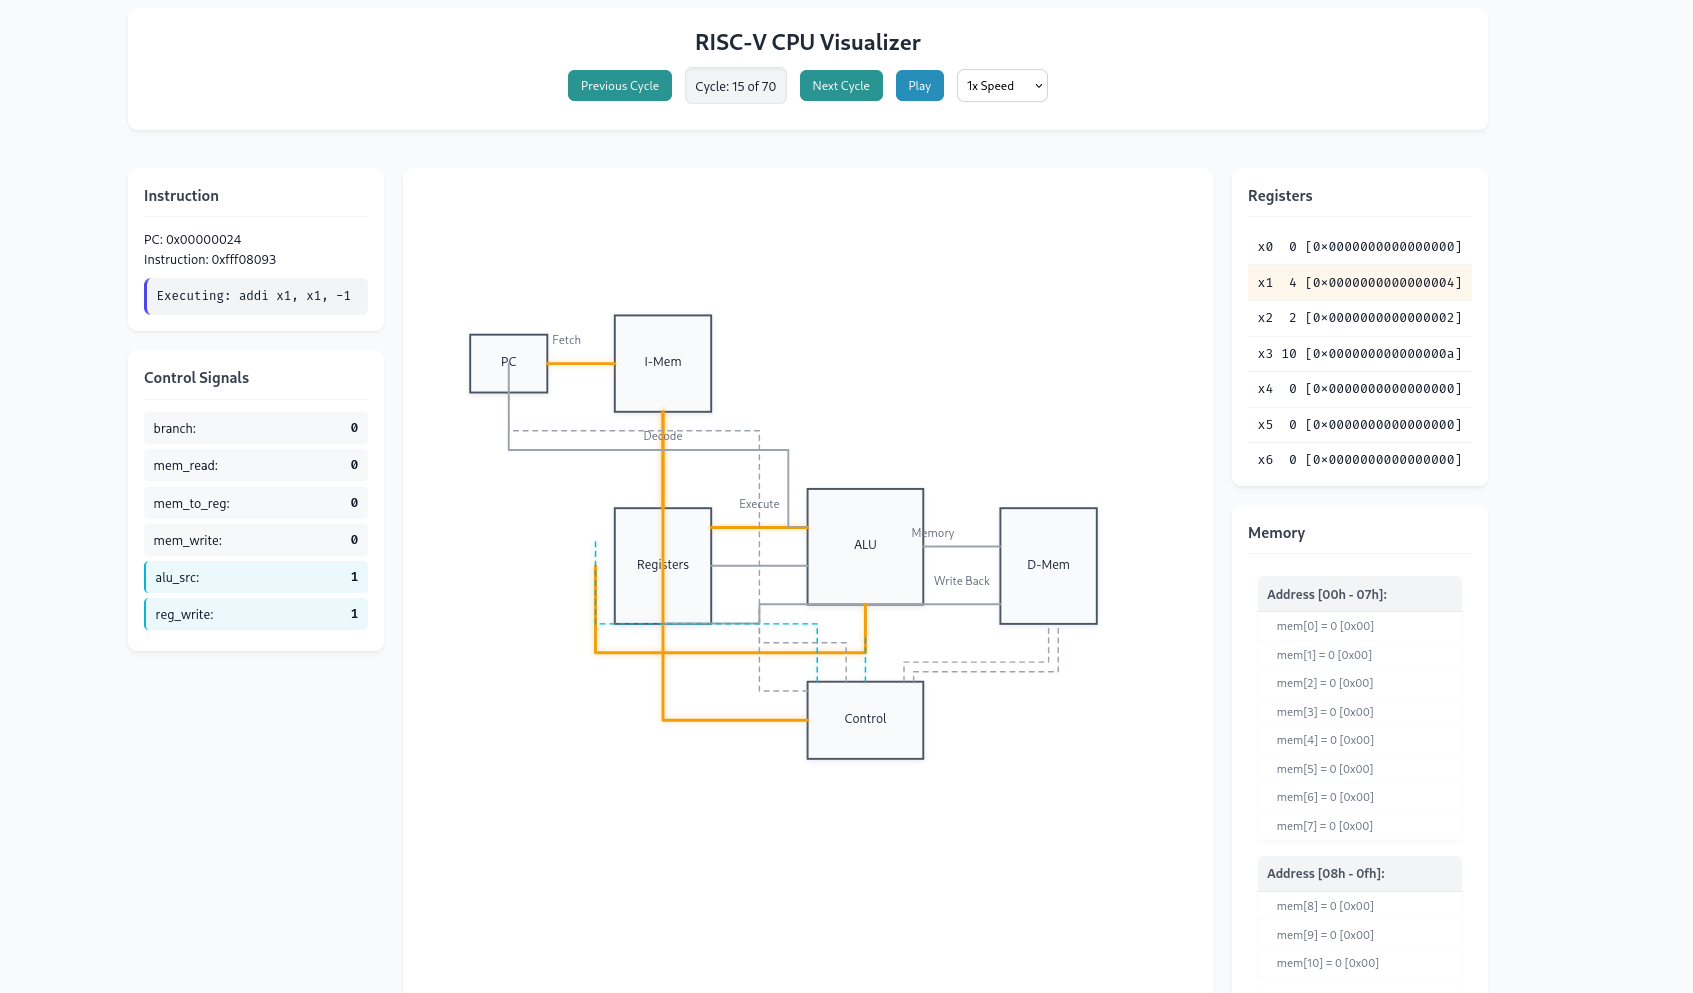
\includegraphics[width=0.95\linewidth]{visualization.png}
    \caption{RISC-V CPU Interactive Visualization Interface}
    \label{fig:cpu-visualizer}
\end{figure}


\section{Pipelined CPU Design Documentation}
\subsection{Overview}
This 5-stage pipelined RISC-V CPU implements a RISC-V subset with hazard handling and branch prediction. Key components are organized into Instruction Fetch (IF), Decode (ID), Execute (EX), Memory Access (MEM), and Write-Back (WB) stages connected through pipeline registers. This design is largely based on principles and architectures described in \citet{ref:harris} and \citet{Patterson:2020}. The control sequence was designed keeping in mind the standard 5-stage pipeline operation.
\begin{figure}[H]
    \centering
    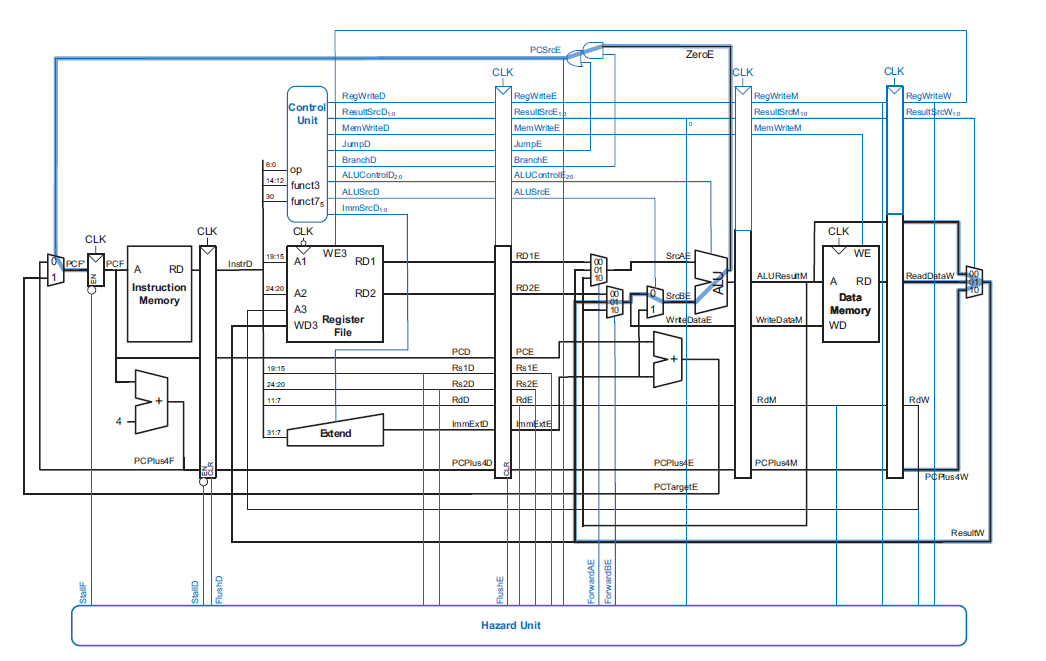
\includegraphics[width=0.95\textwidth]{pipeline_design.png}
    \caption{5-Stage Pipeline Architecture with Forwarding Paths}
    \label{fig:pipeline}
\end{figure}

\subsection{Pipeline Register Implementation}

Four pipeline registers manage intermediate results between stages which are:
\begin{itemize}
    \item \textbf{IF/ID Register}: Stores PC value and fetched instruction

    Inserts NOPs during stalls/flushes. The enable signal \texttt{en} controls the register update, active when not stalled or during branch prediction, and also if stalled in the last cycle to ensure forward progress after a stall ( this has to be done for load hazard) .
    \item \textbf{ID/EX Register}: Preserves control signals and decoded operands

    This register captures the decoded instruction information and control signals, forwarding them to the EX stage. The enable signal \texttt{en} is similar to IF/ID, ensuring data is held during stalls but progresses otherwise .
    \item \textbf{EX/MEM Register}: Carries ALU results and memory addresses

    This register stores the results from the EX stage, such as ALU results, data for memory operations, and control flags, for use in the MEM stage. It is always enabled (\texttt{en} is 1'b1) as it needs to pass data every cycle when the pipeline is not flushed by reset. ( Why enable always you might ask? Because we need to pass the data every cycle and we don't want to stop the data flow in the pipeline and in our design choice we decided to pass (addi x0 x0 0) which is actually the instruction that RISC-V Uses.)

    \begin{figure}[H]
        \centering
        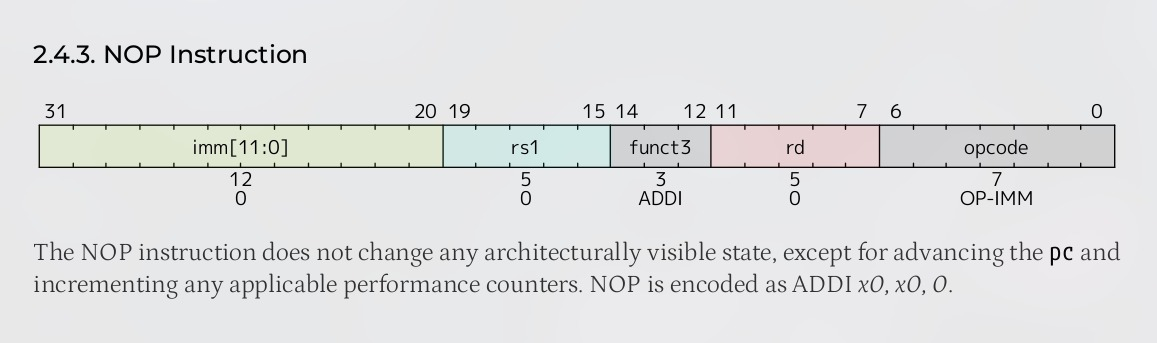
\includegraphics[width=0.95\textwidth]{addix0.jpg}
        \caption{Stalling Instruction in RISC-V}
        \label{fig:addix0}
    \end{figure}
    
    \item \textbf{MEM/WB Register}: Holds data for write-back operations
   
    This register carries data from the MEM stage to the WB stage, including memory read data and ALU results, for the final write-back to the register file. Similar to EX/MEM, it's also always enabled to ensure data progresses in the pipeline. 

\end{itemize}
\subsection{Architectural Rationale and Implementation Details}
\subsubsection{Pipeline Register Design Strategy}
\begin{itemize}
\item \textbf{Naming Convention}: Registers named \texttt{<stage1>\_<stage2>\_register} indicate inter-stage boundaries (e.g., IF/ID separates Fetch/Decode)
\item \textbf{Data Preservation}: Each register stores complete stage output:
\begin{lstlisting}[style=verilog-style]
// EX/MEM register contents
input [63:0] id_ex_pc, alu_result, operandB, branch_target;
input [31:0] id_ex_instruction;
input id_ex_zero, id_ex_branch, id_ex_mem_read, ... ;\end{lstlisting}
    As illustrated, the \texttt{ex\_mem\_register} module (and similarly for others) bundles all necessary outputs from the EX stage needed by subsequent stages. This includes the program counter, ALU result, operand B, branch target, instruction itself, zero flag, and control signals related to branch, memory read/write, memory to register transfer and register write operations.

\item \textbf{Flush/Stall Handling}: Reset or inject NOPs during control hazards. The \texttt{reset} and \texttt{flush} inputs are used to clear pipeline registers during control hazards or at system reset. For data hazards, specifically load-use hazards, NOP instructions are injected into the pipeline to create a stall cycle, as evident in the IF/ID register instantiation:
\begin{lstlisting}[style=verilog-style]
wire [31:0] instr_to_use = flush ? 32'h00000013 : instruction;  // NOP when flush
if_id_register if_id(
    // ...
    .d({
        pc_current,
        stall & ~stalled_last_cycle ? 32'h00000013 : instr_to_use, 
        stall & ~stalled_last_cycle ? 1'b1 : nop_instruction,
        branch_predicted,
        predicted_pc
    }),
    // ...
);\end{lstlisting}
    Here, when a stall condition is detected and it's not a continued stall from the last cycle, a NOP instruction (32'h00000013, which is addi x0, x0, 0) is inserted into the IF/ID pipeline register. As discussed before in  \ref{fig:addix0}, this instruction is used to stall the pipeline for one cycle to resolve load-use hazards.

\end{itemize}
\subsubsection{Control Signal Propagation}
\begin{itemize}
\item \textbf{Stage-Specific Generation}: Control signals originate in ID stage. The \texttt{control\_unit} module is instantiated in the ID stage and generates control signals based on the decoded instruction from the IF/ID register:
\begin{lstlisting}[style=verilog-style]
control_unit ctrl(
    .instruction(if_id_instruction),
    .branch(branch),
    .mem_read(mem_read),
    .mem_to_reg(mem_to_reg),
    .mem_write(mem_write),
    .alu_src(alu_src),
    .reg_write(reg_write)
);\end{lstlisting}

\item \textbf{Pipeline Carry-Through}: Signals propagate with instruction flow. The control signals generated in the ID stage, such as \texttt{branch}, \texttt{mem\_read}, \texttt{mem\_write}, \texttt{mem\_to\_reg}, \texttt{reg\_write}, and \texttt{alu\_src}, are then passed into the ID/EX pipeline register:
\begin{lstlisting}[style=verilog-style]
id_ex_register id_ex(.d({..., branch, mem_read, ...}));\end{lstlisting}
    These control signals then move down the pipeline with the instruction, being registered in subsequent pipeline registers (EX/MEM, MEM/WB if needed for later stages).
\end{itemize}
\subsubsection{Data Hazard Resolution System}
\begin{table}[H]
\centering
\caption{Hazard Handling Mechanisms}
\begin{tabular}{lll}
\textbf{Hazard Type} & \textbf{Detection Method} & \textbf{Resolution} \\
\hline
Load-Use & ID stage register dependency check & 1-cycle stall \\
Data Hazards (EX \ MEM) & Forwarding logic in EX stage & Forwarding \\
Control & Branch misprediction in EX stage & Pipeline flush \\
\end{tabular}
\end{table}
\subsubsection{Branch Prediction Implementation}

\begin{itemize}
\item \textbf{Static Prediction}: Our processor implements a simple static branch prediction strategy.

\begin{lstlisting}[style=verilog-style]
assign branch_predicted = is_branch;\end{lstlisting}

    This line implements an "always-taken" prediction policy. When an instruction is identified as a branch (by checking if its opcode matches the RISC-V branch opcode \texttt{7'b1100011}), we predict it will be taken. This detection happens early in the Instruction Fetch stage:

    \begin{lstlisting}[style=verilog-style]
        wire is_branch = (instruction[6:0] == 7'b1100011);        
    \end{lstlisting}

\item \textbf{Target Calculation}: For predicted-taken branches, we calculate the target address immediately:

\begin{lstlisting}[style=verilog-style]
wire [63:0] if_branch_target = pc_current + if_branch_offset;\end{lstlisting}
    
    This calculation occurs during the IF stage, allowing us to redirect the PC without waiting for later stages. The branch offset is extracted and sign-extended from the instruction according to the RISC-V B-type format:
    
    \begin{figure}[H]
        \centering
        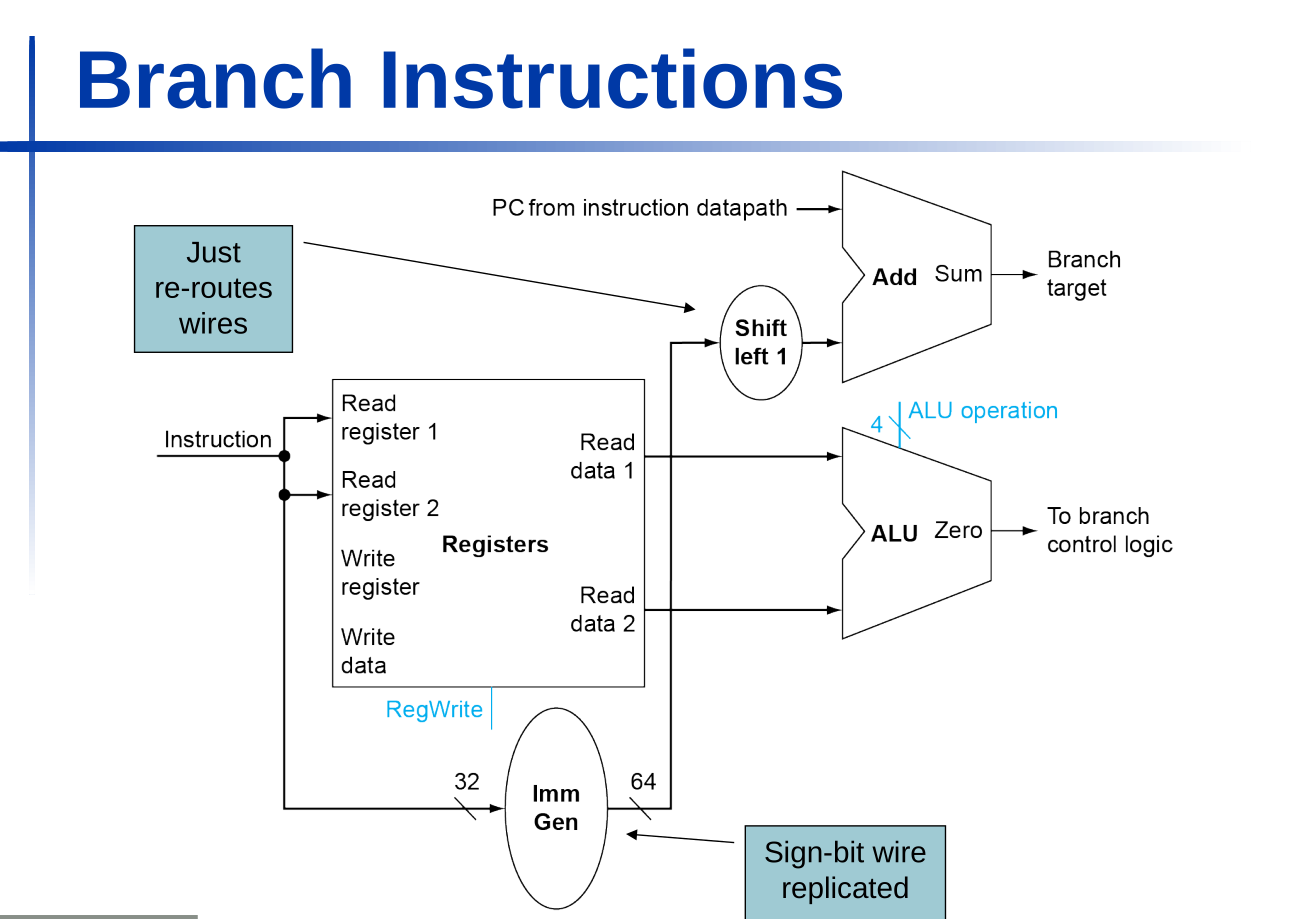
\includegraphics[width=0.6\linewidth]{branchshift.png}
        \caption{Branch Offset Calculation}
        \label{fig:branch-offset}
    \end{figure}
    
\item \textbf{Misprediction Recovery}:

\begin{lstlisting}[style=verilog-style]
assign flush = branch_mispredicted & ~id_ex_branch_predicted;\end{lstlisting}

    This critical line determines when to flush the pipeline after a branch misprediction. 
    
    \begin{itemize}
        \item \texttt{branch\_mispredicted} indicates that the actual branch outcome (determined in EX stage) differs from what was predicted
        \item \texttt{\textasciitilde id\_ex\_branch\_predicted} means the branch was predicted as NOT taken
    \end{itemize}
    
    The combination \texttt{branch\_mispredicted \& \textasciitilde id\_ex\_branch\_predicted} means: "We have a misprediction AND the branch was predicted NOT taken but should have been taken." This specific condition matters because:
    
    \begin{enumerate}
        \item If we predicted a branch as taken but it shouldn't be , we've fetched instructions from the wrong path ( honestly our skill issue ), but we only need to redirect the PC without flushing.
        \item If we predicted a branch as NOT taken but it should be , we've already started executing instructions after the branch that should never execute!!, so we must flush these from the pipeline. THIS IS NUCLEAR and we do it with flush remember from pipeline registers we mentioned we have flush going on all of them hahahahah it gets used now. Indeed Beautiful.
    \end{enumerate}
    
    When the \texttt{flush} signal is asserted, it resets the IF/ID and ID/EX pipeline registers, effectively discarding any incorrectly fetched instructions and allowing execution to continue from the correct path.
\end{itemize}


\subsubsection{Forwarding  Implementation}
\begin{lstlisting}[style=verilog-style]
// EX hazard (ALU result not yet written)
if (ex_mem_reg_write && ex_mem_rd != 0 && ex_mem_rd == id_ex_rs1 && !ex_mem_mem_to_reg)
forwardA = 2'b10;
// MEM hazard (completed execution)
if (mem_wb_reg_write && mem_wb_rd != 0 && mem_wb_rd == id_ex_rs1)
forwardA = 2'b01;\end{lstlisting}
    This Verilog snippet illustrates the forwarding logic for operand A in the EX stage. It checks for RAW hazards by comparing the destination register (\texttt{ex\_mem\_rd}, \texttt{mem\_wb\_rd}) of instructions in the EX/MEM and MEM/WB stages with the source register (\texttt{id\_ex\_rs1}) of the instruction in the EX stage.
    \begin{itemize}
        \item \textbf{EX Hazard Forwarding (2'b10)}: If there's a match with the EX/MEM stage's destination register and it's not a load instruction (indicated by \texttt{!ex\_mem\_mem\_to\_reg}), forward from the EX/MEM ALU result. The condition \texttt{ex\_mem\_rd != 0} ensures that we don't forward if the destination register is x0.
        \item \textbf{MEM Hazard Forwarding (2'b01)}: If there's a match with the MEM/WB stage's destination register, forward from the MEM/WB stage's result. This could be either from memory (\texttt{mem\_wb\_mem\_read\_data} if \texttt{mem\_wb\_mem\_to\_reg} is true) or ALU result. This forwarding path takes precedence over the EX hazard forwarding, ensuring the most up-to-date data is used, especially after a load-use stall is resolved.
        \item \textbf{No Forwarding (default 2'b00)}: If none of the forwarding conditions are met, operand A is read from the register file (\texttt{id\_ex\_reg\_read\_data1}).
    \end{itemize}
    Literally the same logic is implemented for operand B using \texttt{forwardB}.




\subsection{Critical Design Tradeoffs}
\begin{itemize}
\item \textbf{Branch Prediction Simplicity vs Accuracy}: Static always-taken reduces complexity but may increase mispredictions. The choice of always-taken branch prediction is a trade-off favoring hardware simplicity over prediction accuracy. We will further continue to improve this project and add a better branch prediction.

\item \textbf{Forwarding Complexity vs Performance}: Full forwarding network eliminates stalls for Data hazards (except load-use) but increases logic complexity. Implementing a full forwarding network adds complexity to the EX stage and control logic ( which we admit was a skill issue could have implemented a full fledged forwarding network). However, it significantly reduces pipeline stalls due to Data hazards as well, improving overall performance by allowing dependent instructions to proceed without waiting for write-back.

\item \textbf{Stall Mechanism vs Throughput}: Single-cycle load stalls balance pipeline depth with hazard frequency. Introducing a single-cycle stall for load-use hazards is a compromise. It simplifies the hazard detection and resolution logic but may slightly reduce throughput compared to more complex hazard avoidance techniques like load bypassing or more sophisticated stall mechanisms. We looked into those but couldn't implement.

\end{itemize}
\subsection{Key Implementation Nuances}
\subsubsection{Instruction Injection Protocol}
\begin{lstlisting}[style=verilog-style]
// NOP insertion during flush/stall
wire [31:0] instr_to_use = flush ? 32'h00000013 : instruction;
if_id_register if_id(.d({..., stall ? 32'h00000013 : instr_to_use, ...}));\end{lstlisting}
    To handle pipeline flushes (due to branch mispredictions) and stalls (due to load-use hazards), NOP (No Operation) instructions are injected into the pipeline. The code shows that during a flush or stall, the \texttt{instr\_to\_use} signal is assigned the NOP instruction (32'h00000013, which is \texttt{addi x0 x0 0}). This NOP instruction as discussed in Figure~\ref{fig:addix0} is then fed into the IF/ID register, effectively bubbling through the pipeline and ensuring no unintended operations are performed during hazard resolution.

    \subsubsection{Stall State Tracking}
\begin{lstlisting}[style=verilog-style]
reg stalled_last_cycle;
always @(posedge clk) stalled_last_cycle <= stall;\end{lstlisting}
    A register \texttt{stalled\_last\_cycle} is used to track if a stall occurred in the previous clock cycle. This is crucial for the stall mechanism to work correctly for load-use hazards. When a load-use hazard is detected (indicated by the \texttt{stall} signal), the pipeline stalls for one cycle. In the next cycle, even if the hazard condition is still theoretically present (though now resolved by the stall cycle), the pipeline must proceed. The \texttt{stalled\_last\_cycle} flag ensures that the stall is only for one cycle, allowing the pipeline to resume in the subsequent cycle, as reflected in the enable condition of pipeline registers like IF/ID and ID/EX: \texttt{.en(~stall | stalled\_last\_cycle)}.


\subsubsection{End-of-Program Detection}
\begin{lstlisting}[style=verilog-style]
assign end_program = mem_wb_nop_instruction &
~branch_mispredicted &
~branch_predicted;\end{lstlisting}
    The \texttt{end\_program} signal is asserted to indicate the program's termination. It is designed to detect when a NOP instruction reaches the Write-Back stage (\texttt{mem\_wb\_nop\_instruction}) and there are no ongoing branch mispredictions or predictions (\texttt{~branch\_mispredicted \& \~branch\_predicted}). This condition ensures that the program is considered finished only after all instructions, including any NOPs injected due to stalls or flushes, have completed the pipeline and there are no pending control flow changes from branch handling.


\subsection{Architectural Validation Points}
\begin{itemize}
\item \textbf{Forwarding Path Verification}: Validation of all EX/MEM and MEM/WB bypass scenarios confirms the correct data flow and hazard resolution through forwarding.
\item \textbf{Branch Recovery Sequence}: Testing the flush signal timing and PC correction ensures that mispredicted branches are correctly handled, and the pipeline recovers to the correct execution path.
\item \textbf{Load-Use Hazard Handling}: Verification of single-cycle stall insertion confirms that load-use hazards are detected and resolved by stalling the pipeline appropriately, preventing incorrect data usage.
\item \textbf{Control Signal Propagation}: Checking signal integrity through pipeline stages validates that control signals are accurately generated in the ID stage and correctly propagated through subsequent pipeline registers, maintaining control over instruction execution throughout the pipeline.
\item \textbf{Memory Alignment}: Validation of 64-bit data access boundaries ensures that memory operations are correctly aligned, which is critical for data integrity in a 64-bit architecture.
\end{itemize}


\subsection{Simulation}

To validate our pipelined CPU design, we performed extensive testing using a variety of assembly programs. Each test case was designed to verify specific aspects of pipeline functionality, including hazard handling, forwarding, and branch prediction. Ofcourse the Assembler was the same as sequential.

\subsubsection{Case I: Loop with Data Dependencies}

Our first test case exercised both branch prediction and data forwarding capabilities:

\begin{lstlisting}[style=verilog-style]
begin:
    addi x1, x0, 3      # x1 = 3
    addi x2, x0, 7      # x2 = 7

loop:
    beq x1, x0, exit    # if x1==0, end program
    add x2, x2, x1      # x2 = x1 + x2
    addi x1, x1, -1     # x1--
    beq x0, x0, loop    # loop

exit:
    nop
\end{lstlisting}
It validates:
\begin{itemize}
    \item Register forwarding for the \texttt{add x2, x2, x1} instruction which uses updated x1 values
    \item Branch prediction for both conditional and unconditional branches
    \item Control hazard handling when the branch to exit is finally taken
\end{itemize}

Check how the final value in x2 is 13 as expected.

\begin{figure}[H]
    \centering
    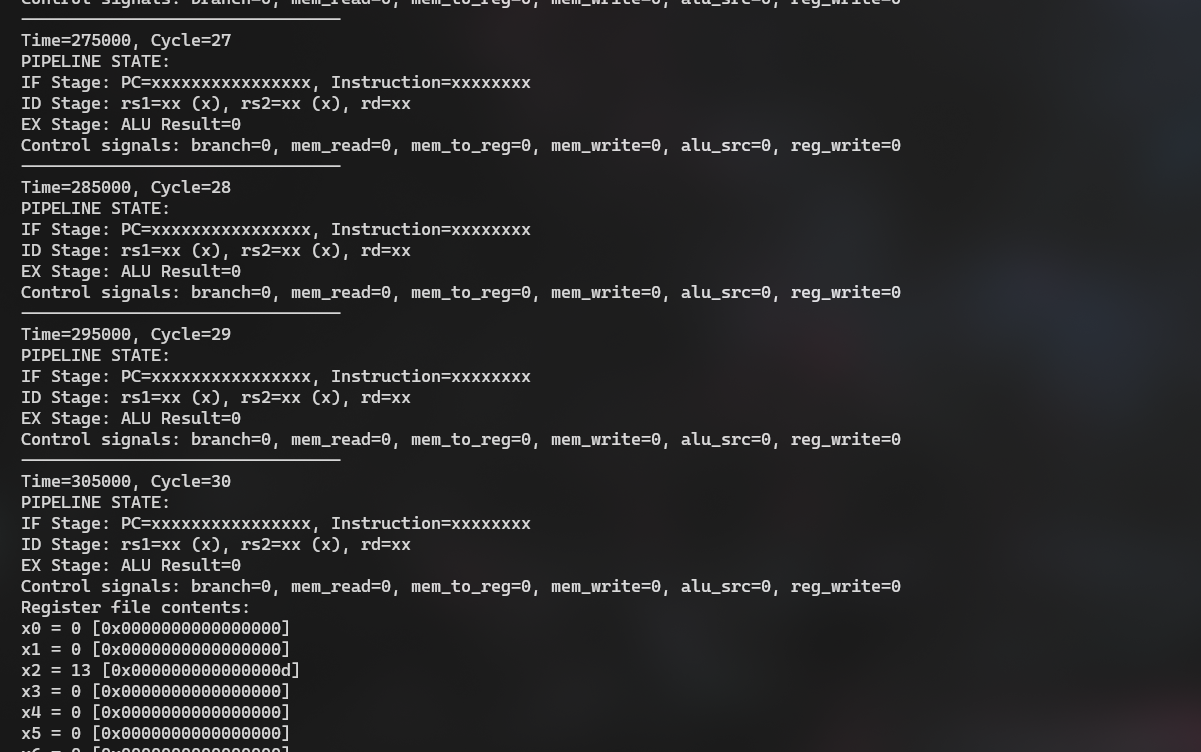
\includegraphics[width=0.95\linewidth]{pipe_test2.png}
    \caption{Loop with Data Dependencies - Pipeline Execution}
    \label{fig:pipe-test2}
\end{figure}






\subsubsection{Case II: Branch Prediction Testing}

A very simple branch testing:

\begin{lstlisting}[style=verilog-style]
begin:
    beq x0, x0, L1
    addi x6, x0, 3

L1:
    addi x5, x0, 4

end:
    nop
\end{lstlisting}

This program includes an always-taken branch at the beginning that skips an instruction. It tests:
\begin{itemize}
    \item Early branch detection in the IF stage
    \item Static "always-taken" prediction implementation check
    \item Correct execution path after branch prediction
\end{itemize}
See how x5 is 4 as expected.

\begin{figure}[H]
    \centering
    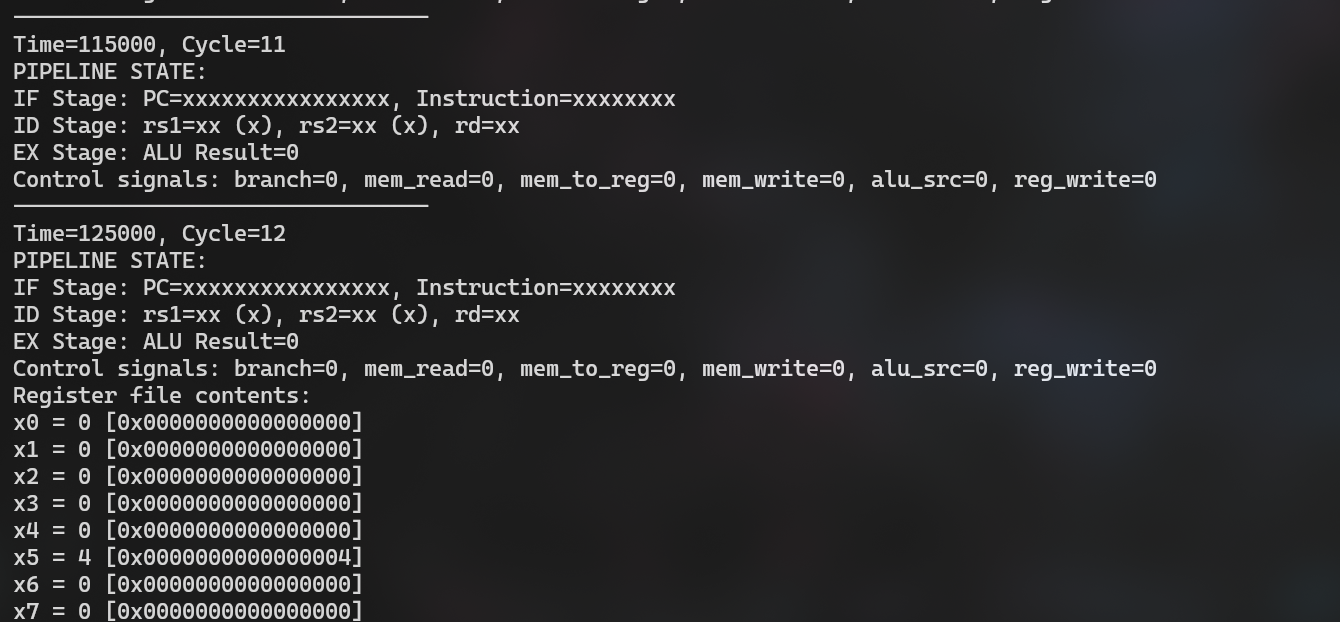
\includegraphics[width=0.95\linewidth]{pipe_test3.png}
    \caption{Branch Prediction Test - Pipeline Execution}
    \label{fig:pipe-test3}
\end{figure}

\subsubsection{Case III: Branch Misprediction Recovery}

Our third test examines pipeline recovery after branch mispredictions:

\begin{lstlisting}[style=verilog-style]
begin:
    beq x0, x0, end

L1:
    addi x5, x0, 4

L2:
    addi x6, x0, 4

L3:
    addi x7, x0, 4

end:
    nop
\end{lstlisting}

This code challenges the pipeline (literally challenged me bro this stuff wasn't working lmao) with multiple branch targets and validates:
\begin{itemize}
    \item Pipeline flush operation when branches are mispredicted
    \item NOP insertion during recovery
    \item PC redirection to the correct execution path
    \item As expected the output shows everything is 0.
\end{itemize}

\begin{figure}[H]
    \centering
    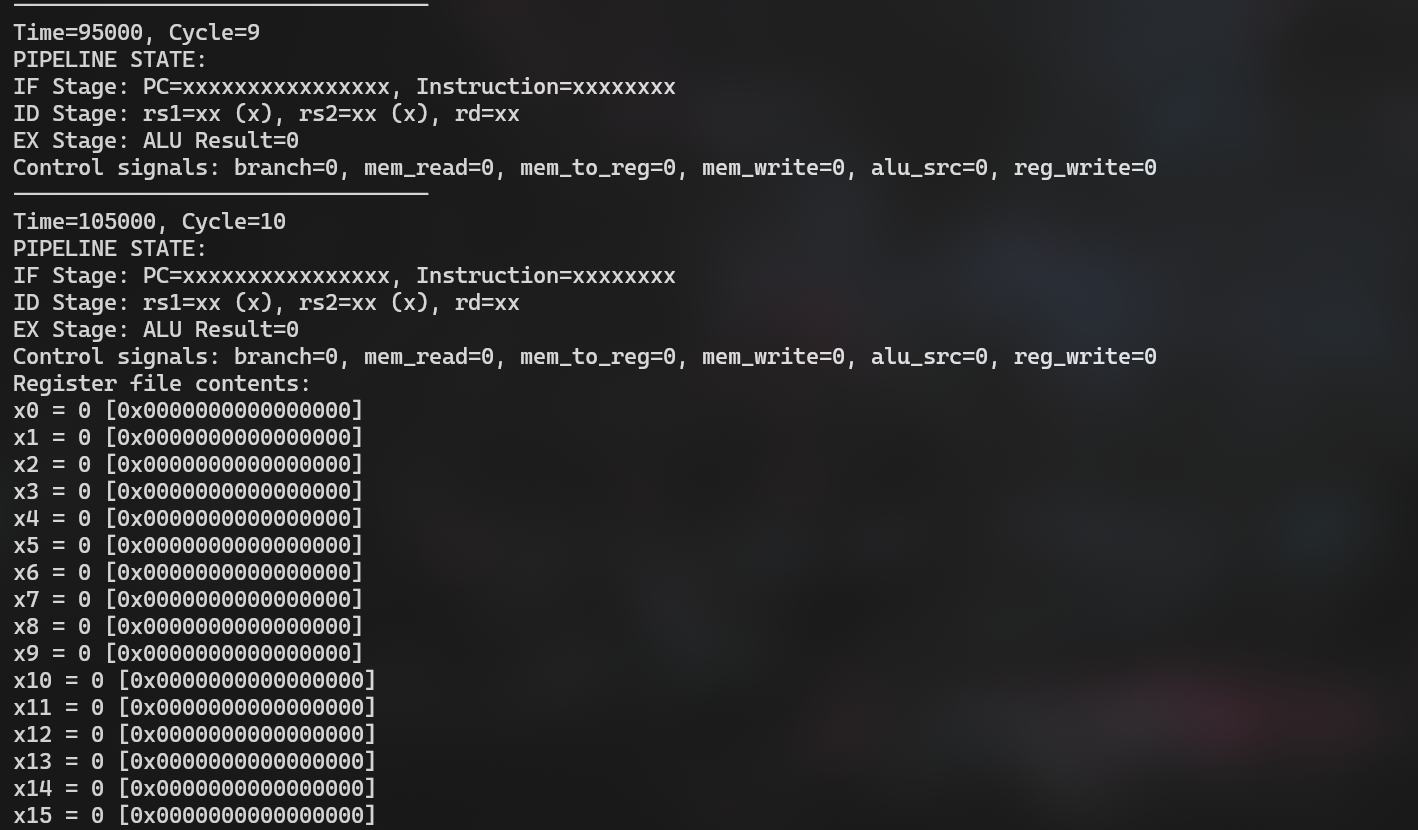
\includegraphics[width=0.95\linewidth]{pipe_test4.png}
    \caption{Branch Misprediction Recovery Test}
    \label{fig:pipe-test4}
\end{figure}

\subsubsection{Case IV: Load-Use Hazard Resolution}

Tests the Load Hazard:

\begin{lstlisting}[style=verilog-style]
begin:
    ld x2, 0(x0)
    addi x4, x2, 1
    add x8, x6, x2
    add x9, x4, x2

end:
    nop
\end{lstlisting}

This code creates a classic load-use hazard where the value loaded into x2 is immediately needed by the next instruction. It confirms:
\begin{itemize}
    \item Accurate detection of load-use dependencies
    \item Proper insertion of a single-cycle stall
    \item Correct resumption of pipeline flow after stall resolution
\end{itemize}

As you can see x0 was loaded with 5 before hand to see this output:
\begin{figure}[H]
    \centering
    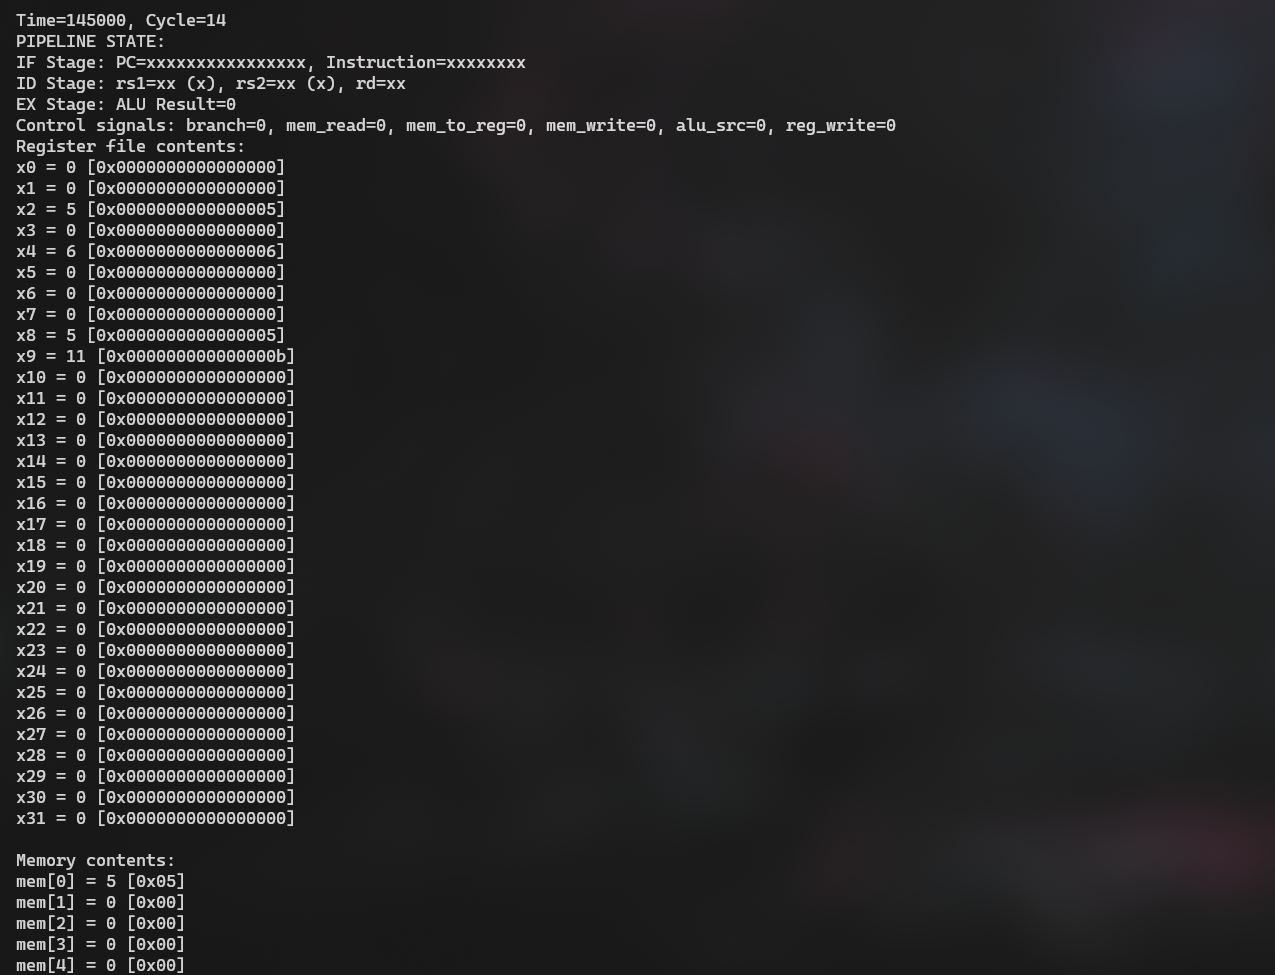
\includegraphics[width=0.95\linewidth]{pipe_test8.png}
    \caption{Load-Use Hazard Resolution Test}
    \label{fig:pipe-test8}
\end{figure}

\subsubsection{Case V: Data Forwarding Validation}

Double Forwarding Test:

\begin{lstlisting}[style=verilog-style]
begin:  
    addi x1, x0, 5
    addi x2, x1, 1
    add x3, x0, x1
    addi x4, x1, 1 

end:
    nop
\end{lstlisting}

The program creates multiple data dependencies in quick succession, ensuring that:
\begin{itemize}
    \item EX-to-EX forwarding works correctly for the result of \texttt{addi x1, x0, 5}
    \item MEM-to-EX forwarding functions for later uses of x1
    \item Forwarding logic properly prioritizes the most recent value as seen by output:
\end{itemize}

\begin{figure}[H]
    \centering
    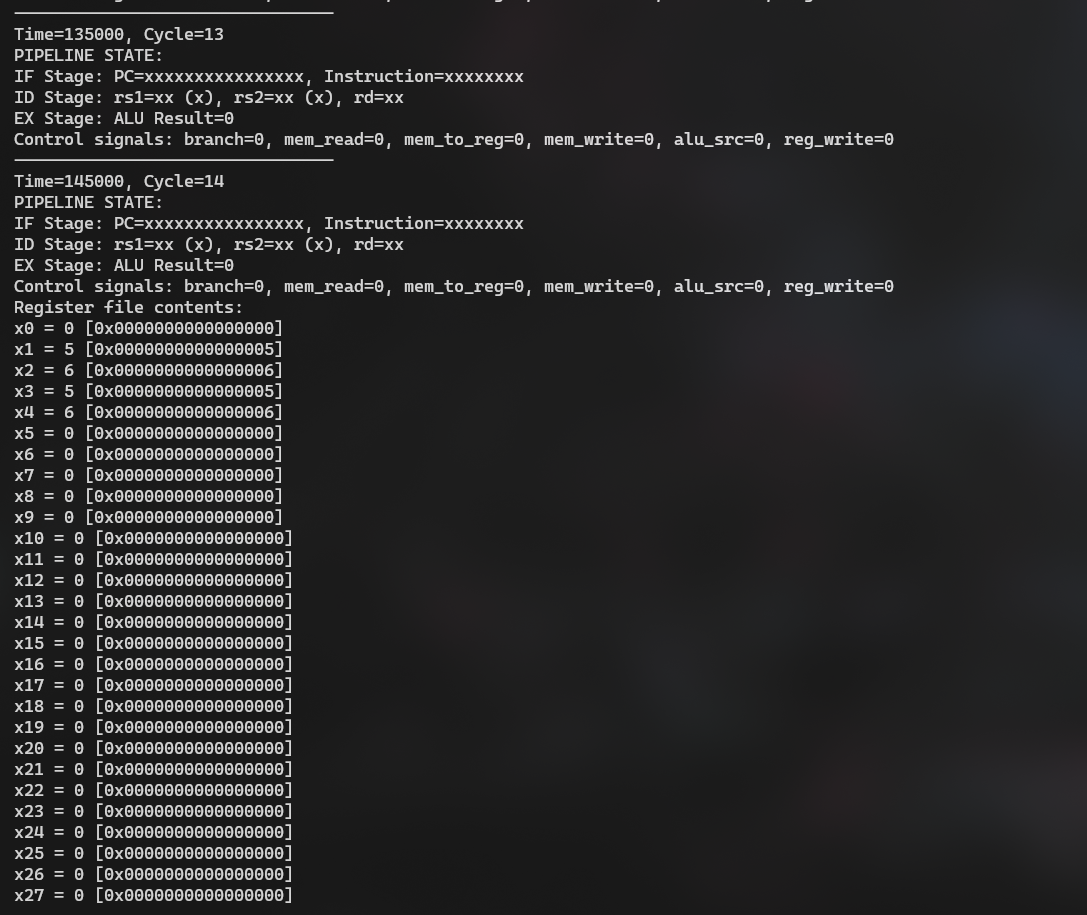
\includegraphics[width=0.95\linewidth]{pipe_test6.png}
    \caption{Data Forwarding Validation Test}
    \label{fig:pipe-test6}
\end{figure}

\subsubsection{Case VI: Control Hazard Complex Case}

ok last test combines branch prediction with data dependencies:

\begin{lstlisting}[style=verilog-style]
begin:
    beq x0, x0, L1
    addi x7, x0, 4
    addi x8, x0, 5
    addi x9, x0, 6
    addi x10, x0, 10

L1:
    addi x5, x0, 4
    addi x6, x0, 5

end:
    nop
\end{lstlisting}

This test validates:
\begin{itemize}
    \item Branch target calculation in the presence of multiple potential paths
    \item Instruction squashing after branch resolution
    \item Resumption of correct execution sequence
\end{itemize}

\begin{figure}[H]
    \centering
    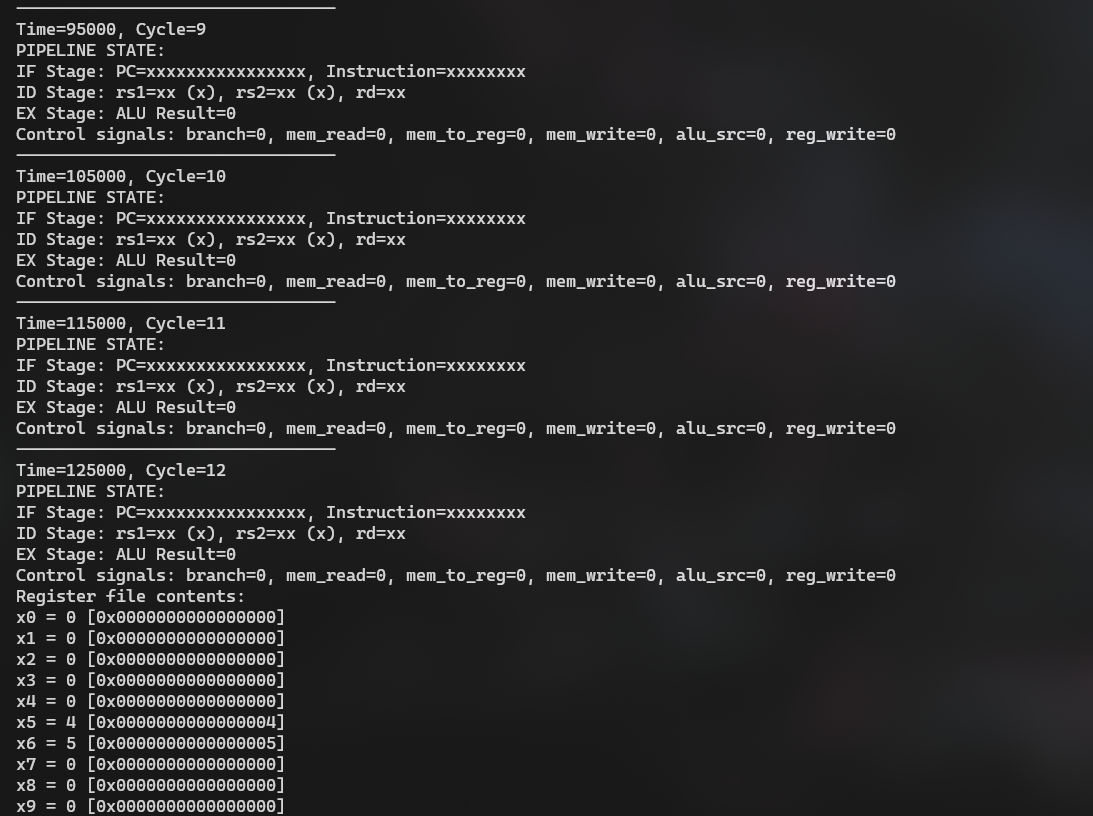
\includegraphics[width=0.95\linewidth]{pipe_test7.png}
    \caption{Control Hazard Complex Test}
    \label{fig:pipe-test7}
\end{figure}

These tests confirm that our pipelined CPU correctly handles the key challenges of pipelined execution: data hazards through forwarding and stalling, and control hazards through prediction and recovery mechanisms.



\section{Contribution and Conclusion}

Well mostly it wasn't a 1/3 split but it was a 9/3 team effort, Hrishikesh worked on report writing , basic structure of Pipelining, desining registers and stuff along with creating beautiful test cases that we have right now , Vignesh the goat made the assembler and ALU , fixed a lot of bugs that we found out on the later stages of testing on even his amazing test cases , he handled the sequential fixes along with Hrishikesh the Data Hazards in pipelining, and for Krish, I finished (which I am writing right now) this last parts of report writing and all the hazards in pipelining along with web view, made the integration for Sequential and all the initial design blocks.

All in all it was more of a team effort so contributing any part to a person feels unjust as all of us worked on almost everything. We would also like to thank Prof Deepak Gangadharan and all the TAs for this amazing of a course, this was really a fun project to work on and we learnt a lot!

We will further work on this on our free time and extend the ISA as much as possible along with better hazard handling strategies that we will come up with. 

Concluding here by saying that our implementation was sophisticated and aligned with the project's best requirements. Hazard handling was graceful, testing will be smoother due to the assembler, and the provided README would make the job much easier. The sequential design had really big programs running while maintaining speed. Future work includes extending the ISA and improving hazard handling strategies.

Adios!! Thanks for Reading
% \section{References}
% \begin{enumerate}
% \item \citet{ref:harris} Harris, D. and Harris, S. (2012). \textit{Digital Design and Computer Architecture}. Morgan Kaufmann.
% \item \citet{Patterson:2020} Patterson, D. and Hennessy, J. (2020). \textit{Computer Organization and Design RISC-V Edition}. Morgan Kaufmann.
% \item Course Slides and Lecture Notes from \textit{Introduction to Processor Architecture}, [Insert Course Name and University, 2024--2025]
% \end{enumerate}


\bibliographystyle{abbrvnat} % You might need to choose a style that fits your needs
\bibliography{references} % Create a references.bib file or adjust the name accordingly

\end{document}
